\documentclass{beamer}

% packages
\usepackage {lmodern}
\usepackage {graphicx}
\usepackage {caption}
\usepackage {colorspace}
\usepackage[LGRgreek]{mathastext}
\usepackage[T1]{fontenc}
\setbeamerfont{footnote}{size=\tiny}
\usepackage[backend=biber, autocite=superscript]{biblatex}
\usepackage {listings}

\lstdefinestyle{customc}{
  belowcaptionskip=1\baselineskip,
  breaklines=true,
  frame=L,
  xleftmargin=\parindent,
  language=bash,
  showstringspaces=false,
  basicstyle=\footnotesize,
  keywordstyle=\bfseries\color{green!40!black},
  commentstyle=\itshape\color{purple!40!black},
  identifierstyle=\color{blue},
  stringstyle=\color{orange},
}

\lstdefinestyle{customasm}{
  belowcaptionskip=1\baselineskip,
  frame=L,
  xleftmargin=\parindent,
  language=bash,
  basicstyle=\footnotesize,
  commentstyle=\itshape\color{purple!40!black},
}

\lstset{escapechar=@,style=customc}


\usetheme[outer/progressbar=foot]{metropolis}
\definecolor{Orange}{HTML}{E87722}
\definecolor{Gray}{HTML}{282A2E}
\setbeamercolor{frametitle}{bg=Orange}

\setbeamertemplate{mini frame}{}
\setbeamertemplate{mini frame in current section}{}
\setbeamertemplate{mini frame in current subsection}{}
\setbeamercolor{section in head/foot}{fg=normal text.bg, bg=Gray}
\setbeamercolor{subsection in head/foot}{fg=normal text.bg, bg=structure.fg}

\makeatletter
\setbeamertemplate{footline}{%
    \begin{beamercolorbox}[colsep=1.5pt]{upper separation line head}
    \end{beamercolorbox}
    \begin{beamercolorbox}{section in head/foot}
      \insertsubsectionnavigationhorizontal{\paperwidth}{}{\hskip0pt plus1filll}\vskip3pt%
    \end{beamercolorbox}%
    \begin{beamercolorbox}[colsep=1.5pt]{lower separation line head}
    \end{beamercolorbox}
}
\makeatother

%\definecolor{optumOrange}{cmyk}{0, .62, .95, 0}
%\setbeamercolor{structure}{fg=optumOrange}


\graphicspath {{images/}}


%\AtBeginBibliography{\scriptsize}

%\setbeamertemplate{bibliography item}{}

\title{Using Vim}
\author{Justin Chao \\ Technology Development Program - Class 11 \\}
\date{November 6, 2017}
\titlegraphic{\hspace*{6cm}
\includegraphics[width=0.4\textwidth, height=0.2\textwidth]{vim}}

\begin{document}
\frame{\titlepage}

\section{Introduction}

\subsection{The Approach}
\begin{frame} {Introduction} {The Approach}
    \begin{itemize}
        \item Introduction \\ 
        \item Basics \\
        \item Getting Stuff Done \\
        \item Advanced Topics
    \end{itemize}
\end{frame}

\subsection{What is Vim}
\begin{frame} {Introduction} {What is Vim}
    Vim is a highly configurable, \underline{modal} text editor built to make creating and changing any kind of text
    very efficient. \\

    \begin{itemize}
        \item System administration\\
        \item Programming\\
        \item Working with HTML, LaTeX, or other markup languages\\
        \item Heavy editing of plain text files\\
    \end{itemize}
\end{frame}

\subsection{Learning Vim}
\begin{frame}[c]{Introduction}{Learning Vim}
    \centering
    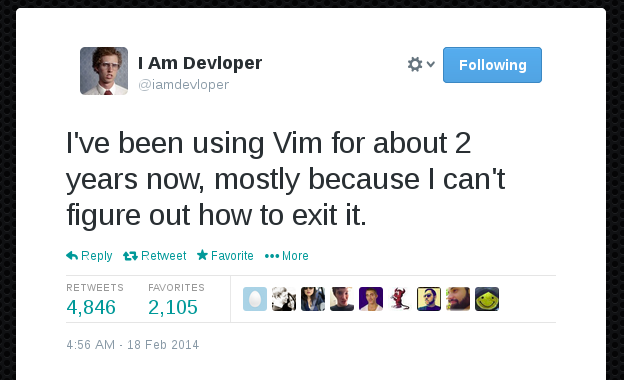
\includegraphics[width=0.8\textwidth]{learningVim}
\end{frame}

\subsection{Why Vim}
\begin{frame} {Introduction} {Why Vim}
    \begin{itemize}
        \item It's ubiquitous. \\It's installed on every Unix-like system, and it's free!\\
        \item It's scalable. \\You can use it just to edit config files or it can become your entire writing platform. \\
        \item It's powerful. \\Because it works like a language vim takes you from frustrated to demigod very quickly. \\
    \end{itemize}
\end{frame}


\subsection{Mastery Levels}
\begin{frame} {Introduction} {Levels to Vim Mastery}
    \begin{itemize}
        \item Level 0: knows nothing about vim \\
        \item Level 1: knows vim basics \\
        \item Level 2: knows visual mode \\
        \item Level 3: knows various motions \\
        \item Level 4: not needing visual mode \\
        \item Level 5: magic things are happening on the screen \\
    \end{itemize}
\end{frame}


\section{Basics}

\subsection{Vim as a Language}
\begin{frame}[c]{Basics}{Vim as a Language}
\begin{table}
    \centering
    \label{tab:label}
    \begin{tabular}{l|c|l}
        Verbs     & d   & delete \\
                  & c   & change           \\
                  & y   & yank (copy)      \\
                  & v   & visually select  \\
        \hline
        Modifiers & i   & inside \\
                  & a   & around \\
                  & NUM & number (1,2,10) \\
                  & t   & searches for something and stops before it \\
                  & f   & searches for that thing and lands on it \\
        \hline
        Nouns     & w   & word \\
                  & s   & sentence \\
                  & p   & paragraph \\
                  & t   & tag (think HTML/XML) \\
                  & b   & block (think programming) \\
    \end{tabular}
\end{table}
\end{frame}


\subsection{Building Sentences}
\begin{frame}[fragile] {Basics} {Building Sentences (Commands)}
    \centering
    Verb - Modifier - Noun

    \begin{lstlisting}[language=sh]
    # delete two words
    d2w

    # change inside sentence
    cis

    # yank (copy) inside paragraph 
    yip

    # change to the < character
    ct<
    \end{lstlisting}
\end{frame}


\section{Getting Stuff Done}

\subsection{File Operations}
\begin{frame}[c]{Getting Stuff Done} {File Operations}
    \begin{table}[htpb]
        \centering
        \begin{tabular}{r|l}
            vi/vim file & open your file in vim \\
            :w & write your changes to the file \\
            :q! & quit vim without saving your changes \\
            :wq & write your changes, and quit \\
        \end{tabular}
    \end{table}
\end{frame}


\subsection{Moving Around}
\begin{frame}[c]{Getting Stuff Done} {Moving Around in Your Text} 
    \begin{table}[htpb]
        \centering
        \begin{tabular}{r|l}
            j & move down one line \\
            k & move up one line \\
            h & move left one character \\
            l & move right one character \\
            gg & go to the top of the file \\
            G & go to the bottom of the file \\
        \end{tabular}
    \end{table}
\end{frame}


\subsection{Moving Within the Line}
\begin{frame}[c]{Getting Stuff Done} {Moving Within the Line} 
    \begin{table}[htpb]
        \centering
        \begin{tabular}{r|l}
            0 & move to the beginning of the line \\
            \$ & move to the end of the line \\
            \^{} & move to the first non-blank character in the line \\
            t" & jump to right before the next quotes \\
            f" & jump and land on the next quotes \\
        \end{tabular}
    \end{table}
\end{frame}


\subsection{Moving by Word}
\begin{frame}[c]{Getting Stuff Done} {Moving by Word} 
    \begin{table}[htpb]
        \centering
        \begin{tabular}{r|l}
            w & move forward one word \\
            b & move back one word \\
            e & move to the end of your word \\
        \end{tabular}
    \end{table}
\end{frame}


\subsection{Searching Your Text}
\begin{frame}[fragile]{Getting Stuff Done} {Searching Your Text} 
    \begin{lstlisting}
    # search for include
    /include<CR>

    # jump forward and land on the < character
    f<

    # jump forward and land right before the < character
    t<

    # change to and including the < character
    ct<
    \end{lstlisting}  
\end{frame}


\subsection{Changing Text}
\begin{frame}[c]{Getting Stuff Done}{Understanding Modes}
    \centering
    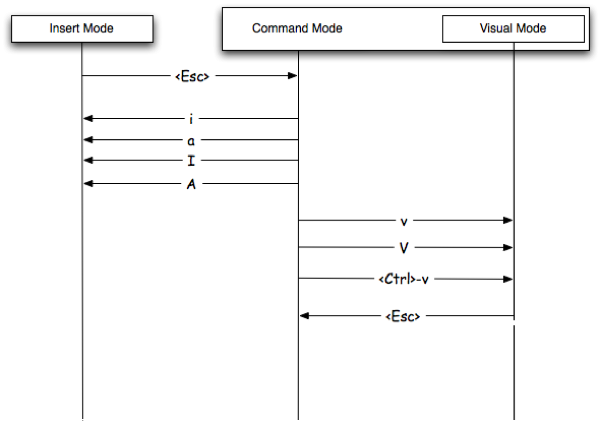
\includegraphics[width=0.8\textwidth]{modes}
\end{frame}


\begin{frame}[c]{Getting Stuff Done}{Inserting Text}
    From Command/Normal mode:
    \begin{table}[htpb]
        \centering
        \begin{tabular}{r|l}
            i & insert before the cursor \\
            I & insert at the beginning of the line \\
            a & append after the cursor \\
            A & append at the end of the line \\
            o & open a new line below the current one \\
            O & open a new line above the current one \\
            r & replace the one character under your cursor \\
            R & replace the character, but stay in insert mode \\
            S & substitute the entire current line \\
            C & delete the line from where you're at, and enter insert mode \\
        \end{tabular}
    \end{table}
\end{frame}


\begin{frame}[c]{Getting Stuff Done}{Deleting Text}
    From Command/Normal mode:
    \begin{table}[htpb]
        \centering
        \begin{tabular}{r|l}
            x    & exterminate (delete) the character under the cursor \\
            X    & exterminate (delete) the character before the cursor \\
            dd   & delete the current line \\
            dt.  & delete from where you are to the period \\
            D    & delete to the end of the line \\
            J    & join the current line with the next one \\
                 & (delete what's between) \\
        \end{tabular}
    \end{table}
\end{frame}


\begin{frame}[c]{Getting Stuff Done}{Undo and Redo}
    \begin{table}[htpb]
        \centering
        \begin{tabular}{r|l}
            u      & undo your last action \\
            Ctrl-r & redo the last action \\
        \end{tabular}
    \end{table}
\end{frame}


\section{Advanced Topics}

\subsection{Repeatability}
\begin{frame}[c]{Advanced Topics}{Repeatability}
    \centering
    "." \\
    \vspace{1cm}
    Given a discreet movement action, combine it with a repeatable command captured in the ".".
\end{frame}

\subsection{Substitution}
\begin{frame}[fragile]{Advanced Topics}{Substitution}
    \begin{lstlisting}
    # change "foo" to "bar" on every line
    :%s/foo/bar/g

    # change "foo" to "bar" on just the current line
    :s/foo/bar/g
    \end{lstlisting}
\end{frame}


\subsection{Text Objects}
\begin{frame}[c]{Advanced Topics}{Text Objects}
    \centering
    word text objects \\
    double quotes \\
    single quotes \\
    parenthesis \\
    paragraphs \\
    back tics \\
    brackets \\
    braces \\
    tags \\
\end{frame}



\subsection{Visual Mode}
\begin{frame}[t]{Advanced Topics}{Using Visual Mode}
    Visual mode magnifies the power of everything we've learned so far, \\
    by allowing you to apply commands to the text that's currently highlighted.

    \begin{table}[htpb]
        \centering
        \begin{tabular}{r|l}
            v      & character based \\
            V      & lined based \\
            vi(    & select inside of parenthesis \\
            vi[    & select inside of brackets \\
            Ctrl-v & coluumn based \\
        \end{tabular}
    \end{table}
\end{frame}


\subsection{Macros}
\begin{frame}[c]{Advanced Topics}{Using Macros}
    \begin{table}[htpb]
        \centering
        \begin{tabular}{r|l}
            qa & start recording a macro named "a" \\
            q  & stop recording \\
            @a & play back the macro \\
        \end{tabular}
    \end{table}

    \begin{enumerate}
        \item Search within the line for "widget" \\
        \item Go to the end of the word and add "-maker" \\
        \item Go to the beginning of the line and add a colon \\
        \item Go to the end of the line and add a period \\
        \item Delete any empty spaces at the end of the line \\
    \end{enumerate}
\end{frame}


\subsection{Plugins}
\begin{frame}[c]{Advanced Topics}{Using Plugins}
    \begin{table}[htpb]
        \centering
        \begin{tabular}{r|l}
            tpope/vim-surround & all about the "surroundings"!  \\
            tpope/vim-fugitive & a Git wrapper \\
            scrooloose/nerdcommenter & easy commenting \\
            scrooloose/nerdtree & a tree explorer plugin \\
            junegunn/fzf & a general-purpose fuzzy finder \\
        \end{tabular}
    \end{table}
\end{frame}


\subsection{Configuring Vim}
\begin{frame}[c]{Advanced Topics}{Configuring Vim}
    \centering
    creating and modifying your .vimrc file
\end{frame}


\section{Resources}
\begin{frame} {Additional Resources}
    \begin{table}[htpb]
        \centering
        \begin{tabular}{r|l}
            vimtutor & built-in tutor to get your started \\
            vim-adventures.com & game based tutorial \\
            github.com/j-chao/dotfiles & my .vimrc \\
        \end{tabular}
    \end{table}
\end{frame}


\end{document}
